%\documentclass[letterpaper,peerreview,12pt,compsoc,draftcls]{IEEEtran}
%\documentclass[10pt,twocolumn,letterpaper]{article}
\documentclass[letterpaper]{article}

%
% Final Checklist TODO XXX 
% - Spellcheck
% - check xxx's todo's etc
%
%\usepackage{ruler}
%\usepackage{cvpr}
%\usepackage{iccv}
\usepackage{times}
\usepackage{epsfig}
\usepackage{graphicx}
\usepackage{amsmath}
\usepackage{amssymb}
%\usepackage{amsthm}
\usepackage{mathtools,empheq}
\usepackage[tight,footnotesize]{subfigure}
%\usepackage{caption}
\usepackage{verbatim}
\usepackage{color}
\usepackage{nomencl}
\usepackage[nocompress]{cite}
\usepackage[pagebackref=true,breaklinks=true,letterpaper=true,colorlinks,bookmarks=false]{hyperref}
\usepackage{algorithm}
\usepackage{enumerate}
\usepackage{multirow}
\usepackage[width=122mm,left=12mm,paperwidth=146mm,height=193mm,top=12mm,paperheight=217mm]{geometry}


\newcommand{\intinf}{\int_{-\infty}^{\infty}}
\newcommand{\argmin}{\operatornamewithlimits{argmin}}

\newcommand{\grad}{\nabla}
\newcommand{\slant}{\sigma}
\newcommand{\R}{\mathbb{R}} % the reals
\newcommand{\skewm}[1]{{#1}_\times}

\renewcommand{\vec}[1]{\mathbf{#1}}

\newcommand{\lbar}{\overline}

\newcommand{\id}{\text{\emph{I}}}
\newcommand{\ransac}{\textsc{ransac}}
\newcommand{\sift}{\textsc{sift}}
\newcommand{\klt}{\textsc{klt}}
\newcommand{\svd}{\textsc{svd}}
\newcommand{\sfm}{\textsc{sfm}}


\newtheorem{thm}{Theorem}
\newtheorem{lem}[thm]{Lemma}

%\newtheorem{theorem}{Theorem}[section]
%\newtheorem{corollary}[theorem]{Corollary}
\newtheorem{corolary}[theorem]{Corollary}
%\newtheorem{proposition}[theorem]{Proposition}
%\newtheorem{lemma}[theorem]{Lemma}

%\theoremstyle{definition}
%\newtheorem{definition}{Definition}
%\newtheorem{remark}{Remark}[section]
\newtheorem{assumption}{Assumption}[section]
%\newtheorem{problem}{Problem}[section]
%\newtheorem{question}{Question}[section]
%\newtheorem{property}{Property}
\newtheorem{transformation}{Transformation}

\numberwithin{equation}{section}

\newcommand{\Gama}{\boldsymbol{\Gamma}}
\newcommand{\gama}{\boldsymbol{\gamma}}
\newcommand{\bsigma}{\boldsymbol{\sigma}}
%\newcommand{\Gama}{\Gamma}
%\newcommand{\gama}{\gamma}
\newcommand{\T}{\boldsymbol{T}}
\newcommand{\N}{\mathbf{N}}
\newcommand{\NSurface}{\mathbf{N}}
\newcommand{\Nlocal}{\overline{\N}} % normal in local coordinates
\newcommand{\balpha}{\boldsymbol{\alpha}}
\newcommand{\tDt}{t+\Delta t}
\newcommand{\bpsi}{\boldsymbol{\boldsymbol{\psi}}}
\newcommand{\bp}{\mathbf p}
\newcommand{\deldt}[1]{\frac{\partial#1}{\partial t}}
\newcommand{\ddt}[1]{\frac{d #1}{dt}}
\newcommand{\delds}[1]{\frac{\partial#1}{\partial s}}
\newcommand{\mybar}[1]{\overline{#1}}
\newcommand{\norm}[1]{\|#1\|}
\newcommand{\I}{\mathbf{I}}
\newcommand{\brho}{\boldsymbol{\rho}}
\newcommand{\lightrgb}{\boldsymbol{l}}
\newcommand{\B}{\boldsymbol{B}}
\renewcommand{\t}{\boldsymbol{t}}
\newcommand{\n}{\boldsymbol{n}}
\renewcommand{\b}{\boldsymbol{b}}
\newcommand{\e}{\boldsymbol{e}}
\newcommand{\f}{\boldsymbol{e}_3}
\newcommand{\ff}{\mathbf{f}}
\newcommand{\hf}{\boldsymbol{\hat{f}}}
\newcommand{\g}{\boldsymbol{g}}
\newcommand{\G}{\boldsymbol{G}}
\newcommand{\bc}{\boldsymbol{c}}
\newcommand{\Curve}{\Gamma}
%\newcommand{\X}{\boldsymbol{X}}
%\newcommand{\x}{\boldsymbol{x}}
\newcommand{\X}{\mathbf{X}}
\newcommand{\x}{\mathbf{x}}
\newcommand{\tilx}{\tilde x}
\newcommand{\tily}{\tilde y}
\newcommand{\tilgama}{\tilde \gama}
\newcommand{\ugama}{\hat{\gama}} %unit gama
\newcommand{\br}{\bar r}
\newcommand{\Kc}{\mathbf K_c}
\newcommand{\Kim} {\mathcal K_{im}}
\newcommand{\lepi}{\mathbf r}
\newcommand{\itan}{\tan^{-1}}
\newcommand{\uu}{\xi}
\newcommand{\buu}{\bar \uu}
\newcommand{\bvv}{\bar \vv}
\newcommand{\vv}{\eta}
\newcommand{\VV}{\mathbf{V}} % translational velocity
\newcommand{\VVspeed}{V} % translational velocity
\newcommand{\field}{\boldsymbol\chi}
\newcommand{\ufield}{\hat{\boldsymbol{\chi}}}
\newcommand{\fieldc}{\chi} % field component
\newcommand{\transl}{\mathcal{T}}
\newcommand{\rot}{\mathcal{R}}
\newcommand{\albedo}{\alpha}
\newcommand{\depth}{\rho}      % depth as z
\newcommand{\udepth}{{\hat{\rho}}} % depth along ray
\newcommand{\ttransl}{\T} % translation tangent
\newcommand{\surface}{\mathcal{M}} % surface/manifold
\newcommand{\surf}{\mathcal{M}} % surface/manifold short
\newcommand{\jacm}{\mathtt{J}} % Jacobian matrix
\newcommand{\xbar}{\bar x}
\newcommand{\ybar}{\bar y}
\newcommand{\zbar}{\bar z}

\newcommand{\bdelta}{\boldsymbol \delta}
%\newcommand{\X}{\boldsymbol{X}}
%\newcommand{\x}{\boldsymbol{x}}
%\newcommand{\X}{\mathbf{X}}
%\newcommand{\x}{\mathbf{x}}
\newcommand{\boldu}{\mathbf{u}}
\newcommand{\boldv}{\mathbf{v}}
\newcommand{\boldw}{\mathbf{w}}
% The following are not very good constructs it seems. Better to use just
% \begin{bmatrix}..\end{\bmatrix}
\newcommand{\datsqbr}[2][rrrrrrrrrrrrrrrrrrrrrrrrrrrrrrrrrrrr]{\left[
\begin{array}{#1}
#2\\
\end{array}
\right]
}
\newcommand{\tgtveloc}{\tilde\alpha} % real tangential velocity
\newcommand{\trace}{\text{trace}\,}
\newcommand{\benx}{x} % ben's aux. variable in da calibration paper

\newcommand{\ie}{{\it i.e.}}
\newcommand{\etc}{{\it etc}}
\newcommand{\eg}{{\it e.g.}}
\newcommand{\wrt}{{\it w.r.t. }}
\newcommand{\etal}{{\it et.~al.}}


\usepackage{url}
\usepackage{graphicx}
\usepackage[tight,footnotesize]{subfigure}
\usepackage{color}
\usepackage{verbatim}
\usepackage[pagebackref=true,breaklinks=true,letterpaper=true,colorlinks,bookmarks=false]{hyperref}

%%%%%%%%%%%%%%%%%%%%%%%%%%%%%%%%%%%%%%%%
% You have two versions of the macro
% \draftnote{My note}. The first version puts notes (e.g. My note in the example)
% into the margin of your document. The second formats the note as nothing. You
% 'comment out' the version of the macro you don't want (using a % at the
% beginning of the line).
%\newcommand{\draftnote}[1]{\marginpar{\tiny\raggedright\textsf{\hspace{0pt}#1}}}
\newcommand{\draftnote}[1]{\marginpar{\tiny\raggedright\textsf{\hspace{0pt}#1}}}
%\newcommand{\draftnote}[1]{}

% This one is just for the comments for in-line text.
\newcommand{\indraftnote}[1]{\textcolor{blue}{\texttt{\footnotesize[#1]}}}
\newcommand{\todo}[1]{\indraftnote{todo: #1}}
%\newcommand{\indraftnote}[1]{}


\begin{document}
\title{%
AA Distributed Software Development Methodology
}

\author{%
Renato~Fabbri \and Ricardo~Fabbri \and Vilson Vieira \and Alexandre Negrao \and Lucas Zambianchi
\and Marcos Mendonca
}

\maketitle
%\thispagestyle{empty}


\begin{abstract}
Algorithmic Autoregulation is a new self-regulating methodology for coordinating
distributed teamwork,  based on collaboration and
individual merit. Team members take on an egalitarian role, and stay
voluntarily logged into so-called AA sessions for part of their time (e.g.,
2h/day), during which they check for open tickets and microblog periodical
"tweets" or status messages they wish to share about their activity with the
team. These status logs are publicly aggregated and are peer-validated,
as in code review, and a public videolog is recorded summarizing daily experiences.
This methodology is well-suited for increasing the efficiency of distributed
teams through asynchronous on-demand communication, reducing the need for
central management, unproductive meetings or time-consuming reports.  The AA
methodology also legitimizes the activities of a distributed software team.  It
thus enables entities to have a solid means to fund these activities, allowing
for new and concrete business models to emerge for very distributed software
development.  
\end{abstract}



\section{Introduction}

One of the defining features of modern times is the widening geographical
distribution of software teams~\cite{}. One example is the free software
movement. \todo{citar alguns exemplos}.

However, we have noticed how difficult it is to coordinate and fund free
software on a larger scale than currently available, when teams are very
heterogeneous containing not only volutaries and very experienced developers,
but also contractors from different backgrounds and cultures.

Another problem faced by modern software companies and other collectives are frequent
ineffective meetings, which are seldom focused to the interest to any
attendant. The result is that it has become the norm to participate in too many
meetings with the laptop open, which is very unproductive at the very least.
Coders like to code, to be productive, to have their hands-on their project to
do what they're best at. They hate to have to stop for too many meetings,
and they hate to have to write lengthy reports to justify their funding.
\todo{ler mais. cacm, etc}

AA is a methodology and an associated software system for coordinating
distributed teamwork.  Team members take on an egalitarian role, and stay
voluntarily logged in the system for part of their time (e.g., 2h/day), during
which they microblog periodical "tweets" about their activity. These microblog
logs are publicly aggregated and are validated by their own peers. Through AA,
we have a methodology and an associated system to validate and enable the
activities of a distributed software team. It implicitly legitimizes financing
the expansions of the team's activity. The AA methodology is specially useful
for coordinating distributed and decentralized teamwork, providing effective
means to asyncrhonously update different team members without the need for
syncrhonous unproductive meetings.

Figure~\ref{fig:mm} summarizes our methodology.


\begin{figure}
\begin{center}
   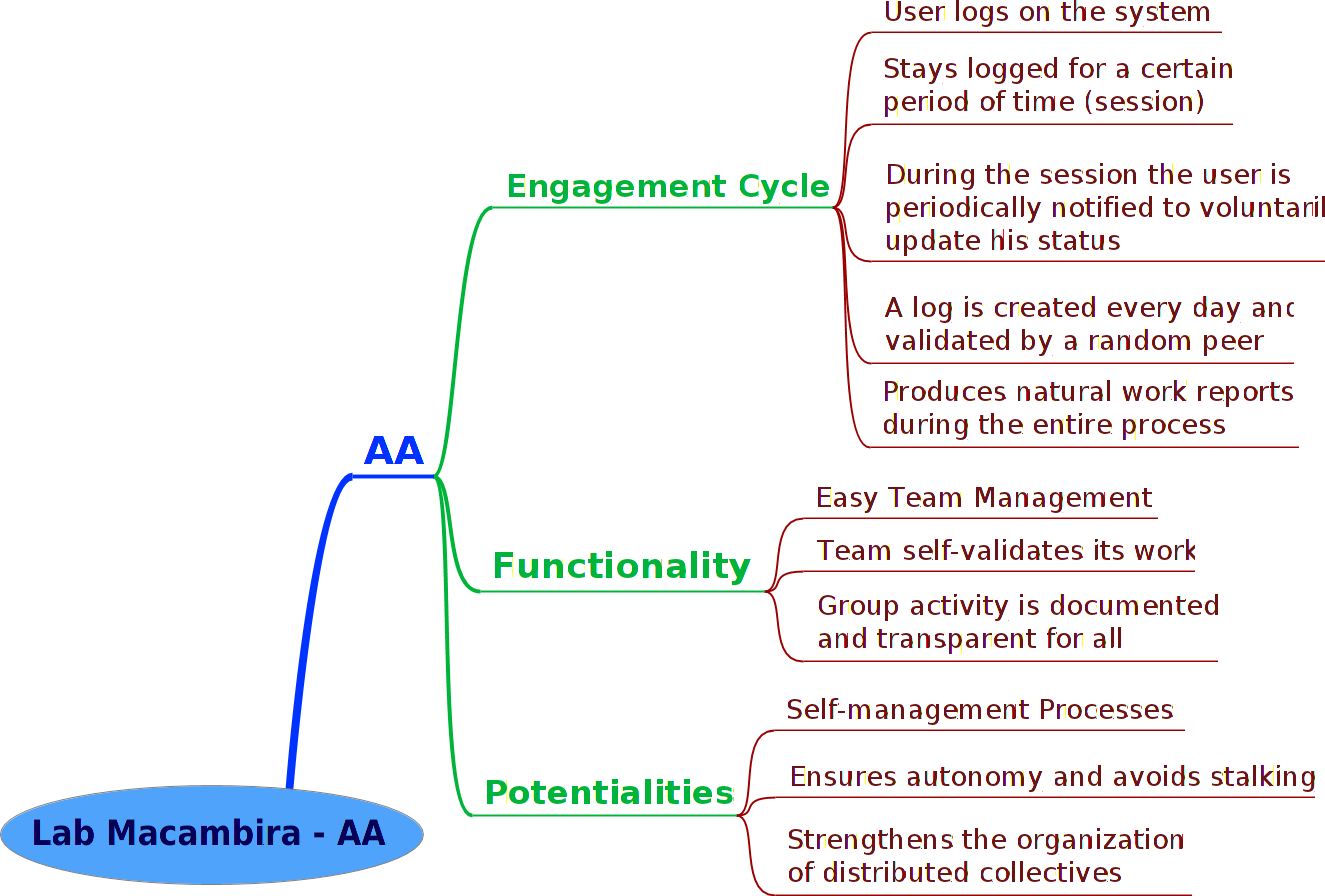
\includegraphics[width=0.8\linewidth,keepaspectratio=true]{figs/aa-mm.png}
\end{center}
   \caption{
   Mindmap of our methodology
   }
\label{fig:mm}
\end{figure}

\todo{alerts work for greater consciousness of time}

\section{Related Work}
\todo{survey other methodologies such as agile etc}
\todo{probably a good source http://agilemanifesto.org/}

\section{The AA Methodology}

\section{AA Session}

From the developer perspective, the AA methodology is based on creating pretty
small high perspective reports of what they're doing in a specific timeframe,
that can be something between 5 to 15 minutes, depending in what is more
confortable for the developer, an AA Session would be a period of at least 2hrs
doing these reports. The developer can set reminders to show up when its time
to make a new report.

The objective of the flexible timeframe and reminders is to don't generate much
overhead for the developer to be in an AA session, so he can make the reports
and also concentrate in his code.

Each report can be sent directly to the an online server, or cached locally in
a log for sending later, this is necessary to make possible for developers that are
offline to use AA without problems.

The developer can also add a screencast in the end of session to make a summary
of what has been done in the session, explaining with his words and showing his
results, possibly making some points more easily understandable then with only
the reports from the AA session.



\section{The AA Methodology}

\section{Conclusion}

%\section*{Acknowledgments}
%The authors would like to thank NSF and CNPq.

%{\small
%\input{paper-draft.bbl}
%%%%\bibliographystyle{splncs}
% this is a good style for drafting
%\bibliographystyle{abstract}
% this is a good style for finals
\bibliographystyle{acm}
\bibliography{personal}
%}

\end{document}
